\documentclass[%
reprint,
amsmath,amssymb,
aps,
]{revtex4-1}
\usepackage{graphicx}% Include figure files
\usepackage{dcolumn}% Align table columns on decimal point
\usepackage{bm}% bold math
\usepackage[utf8]{inputenc}
\usepackage{listings}
\usepackage{amsmath}
\usepackage{physics}
\usepackage{booktabs}
\bgroup
\def\arraystretch{1.3}

\makeatletter
\newcommand*{\rom}[1]{\expandafter\@slowromancap\romannumeral #1@}
\makeatother

\begin{document}
\title{Numerical integration}
\author{Oline A. Ranum}
\affiliation{%
 University of Oslo \\ Institute for physics\\
 olinear@student.matnat.uio.no
}
\date{\today}


\begin{abstract}
	The following experiment was undertaken as a mean to 
\end{abstract}
\maketitle

\section{Introduction}
Wherever you go in science, there is the need to find integrals.
- what are integrals 
-what is numerical integration 
Numerical integration makes estimations  of any integral possible, not just the ones that fit a mathematical framework. 
A broad selection of numerical integration methods has since been developed. 

Monte Carlo methods are widely used in Science, from integration of multi-dimensional integrals to solving ab initio problems in for instance chemistry, physics, medicine or bilogy. Computational finance is one of the novel fields where monte carlo methods have found a new field of applications

\section{Theory}



\subsection{Numerical integration \& the Gaussian quadrature} \noindent 
The basic idea behind all numerical integration methods is to approximate the integral 
\begin{equation}\label{numint}
	I = \int_{a}^{b}f(x)dx \approx \sum_{i=0}^{N-1} \omega_if(x_i)
\end{equation}
where $\omega$ and $x$ are the weights and the chosen mesh points, respectively. Interpolatory quadrature rules, such as Simpson's- or the trapezoidal rule, are based on the assumption that the quadrature points, or nodes, are preassigned equidistantly or with a fixed distribution. The Gaussian quadrature (hereafter GQ) is based on the notion first made by Gauss, that a suitable variation of the nodes would in general lead to a better accuracy [Kythe \& Schaferkotter, 2005]. The core idea of GQ is to have the freedom to choose both the weighting coefficients and the location of the abscissas/nodes at which the function is to be evaluated. One therefore no longer requires the nodes to be equally spaced, and therefore giving twice the number of degrees of freedom in regards to the classical interpolatory quadratures [Press et al. 2007]. As such, many variations and generalizations of the Gaussian formulas have been developed on the form equation \ref{numint}, where the weights $\omega_i$ are positive zeros of certain orthogonal polynomials and the nodes $x_i$ are distinct points in a given interval [Kythe \& Schaferkotter, 2005]. \\
\indent It is important to note that higher order does not necessarily imply higher accuracy. The former only implies the latter in the case where the integrand is very smooth, in the sense that the integrand is well approximated by a polynomial. In the case of a Gaussian quadrature, it is possible to arrange both weights and abscissas to make integrals exact for a class of integrands on the form of polynomials times some known function $W(x)$. One chooses $W(x)$ to remove integratable singularities from the desired integral. As stated in Press et al., given $W(x)$ and an integer N, it is possible to find a set of weights $w_j$ and nodes $x_j$ such that the approximation 
\begin{equation}
	\int_{a}^{b}W(x)f(x)dx \approx \sum_{j = 0}^{N-1}w_jf(x_j)
\end{equation}
is exact if $f(x)$ is a polynomial. [Press et al., 2015]


\subsection{Orthonormal polynomials} \noindent 
The subject of Gaussian quadratures was further developed by Jacobi's derivation of Gauss's work by means of orthogonal polynomials [Press et al. 2007]. A set of polynomials $\{p_i\}$ of degree $i$ is said to be orthogonal with respect to the inner-product if $<p_i, p_j> = 0$ for $i\not = j$ on a finite or infinite interval $[a,b]$. That is, if the powers are orthonormalized, one should obtain a unique set of polynomials $p_i(x)$ of degree $n$ such that
\begin{equation}
	\braket{p_i}{p_j} = 
	\int_{a}^{b} W(x)p_i(x)p_j(x)dx = \delta_{ij} 
\end{equation}
where $\delta_{ij}$ is the Kronecker delta
\begin{equation}
	\delta_{ij} = \left\{
	\begin{array}{ll}
	1 & i = j\\
	0 & i \not =j 
	\end{array} \right\}
\end{equation}
The orthogonality property for polynomials defined in this manner is equivalently defined for a discrete set of polynomials [Kythe \& Schaferkotter, 2005]. Two functions are said to be normalized if its scalar product with itself is unity. A set of functions that are all mutually orthogonal and also all  individually normalized is called an orthonormal set.  [Press et al., 2015]

\subsubsection{Constructing orthogonal polynomial sets}
It is possible to find a set of polynomials through recurrence relations which has the property of beeing mutually orthogonal over a spesified weight function W(x) and that includes exactly one polynomial of order $j$, called $p_j(x)$ for each $j = 0,1,2,\dots$. Such a constructive procedure is described by Press et al.:
\begin{align*}
	p_{-1}(x) &\equiv 0\\
	p_{0}(x) &\equiv 1\\
	p_{j+1}(x) &\equiv (x-a_j)p_j(x)-b_jp_{j-1}(x)\\
\end{align*}
where
\begin{align*}
	a_j &= \dfrac{\braket{xp_j}{p_j}}{\braket{p_j}{p_j}} &\hspace{1mm} j = 0,1, \dots \\ &&\\
	b_j &=\dfrac{\braket{p_j}{p_j}}{\braket{p_{j-1}}{p_{j-1}}} &\hspace{1mm} j = 1,2, \dots
\end{align*}
The coefficient $b_0$ would be arbitrary, and can therefore be set to zero. It can be showen that the polynomial $p_j(x)$ have exactly $j$ distinct roots in a given interval $[a,b]$. \\
The fundamental theorem of Gaussian quadratures then states that the  abscissas of the N point Gaussian quadrature equations with weighting function W(x) in the interval $[a,b]$ are precisely the roots of the orthogonal polynomial $p_N(x)$ for the same interval and weighting function. Once the abscissas are known, one needs to find the weights $w_j$. For classical orthogonal polynomials, such as the Gauss-Legendre and Gauss-Laguerre, the coefficients $a_j$ and $b_j$ have an explicit solution. Thus, the problem reduces to determining the zeros of the polynomial $p_N(x)$, and the computation of the weights [Press et al.]\\

\subsubsection{Computation of abscissas and weights}
Both the Gauss-Legendre and - Laguerre are classical, well-studied, orthogonal polynomials and can be used as good starting guesses. After an initial guess is made, one can apply Newtons method, and expect  it to converge rather rapidly to locate the zero-point. [Press et al.] \\
For the Gauss-Legendre and Gauss-Laguerre the following direct root finding is concidered to be faster by a factor of 3 to 5, than any other method [Press et al.]\\
\textit{Gauss-Legendre}:
\begin{equation*}
	W(x) = 1 \hspace{3mm} -1 < x < 1 
\end{equation*}
\begin{equation}
	(j+1)P_{j+1} = (2j +1)xP_j - jP_{j-1}
\end{equation}
\textit{Gauss-Laguerre}
\begin{equation*}
W(x) = x^\alpha e^{-x} \hspace{3mm} 0 < x < \infty 
\end{equation*}
\begin{equation}
(j+1)L_{j+1}^\alpha = (-x+2j+\alpha+1)L_j^\alpha -(j+\alpha)L_{j-1}^\alpha
\end{equation}
\subsubsection{Newtons method}
Newton's method requires the derivative of the polynomial, which is evaluated by standard relations in terms of $p_N$ and $p_{N-1}$. 

\subsection{Stochastic Monte-Carlo Integration}
The Monte-Carlo integration method 
\begin{equation}
	I = \qty[\int_{a}^{b}f(x) dx]^D = (b-a)^DE[f(x)]
\end{equation}
where D is the number of dimensions
\subsubsection{Probability distribution functions}
The only requirement for many applications of Monte Carlo methods is that a probability distribution function (PDF) is known to describe the physical system. Once a PDF is known a Monte Carlo simulation can proceed by random sampling from the PDF's. 

Since the result is built on the average of many simulations over the number of ovservations, the statical error - the variance - can be predicted. The PDF is a function $p(x)$ on the domain which in the discrete case gives us the probability or relative frequency with which these values of X occure 
\begin{equation}
	p(x) = \textnormal{Prob}(X=x)
\end{equation}
The PDF must satisfy two properties. First, the PDF has tobe nprmalized so that all the probabilities add up to unity
\begin{equation}
	\sum_{x_i\in \mathcal{D}} p(x_i) = 1
\end{equation} 
Assuming that the PDF is normalized, the probability then has to be of a positive nature 
\begin{equation}
	0 \leq p(x) \leq 1
\end{equation}
One especially important PDF is the uniform distribution defined as 
\begin{equation}
	p(x) = \dfrac{1}{b-a}\Theta(x-a)\Theta(b-x)
\end{equation}
where
\begin{align*}
	\Theta(x) &= 0& \hspace{2mm} x < 0\\
	\Theta(x) &= 1& \hspace{2mm} x \geq 0\\
\end{align*}
Another important probability distribution is the exponential distribution 
\begin{equation}
	p(y) = \exp{-y}
\end{equation}
where $p(x)$ is given by the uniform distribution $x\in[0,1]$. Assuming that the probability is conserved through the variable transformation
\begin{equation}
p(y)dy = \exp{-y}dy = dx
\end{equation}
The above definitions is written as functions of a single stochastic variable, and is thereby known as univariante. A PDF consisting of multiple variables is usually refered to as mutlivariante, and the multivariante expectation value is defined similarly as the above univariante case, but all stochastiv variables are taken into account simultaniously on the form
\begin{equation}
	E[f(x_1\dots x_N)] = \int\dots\int f(x_1\dots x_N)P(x_1\dots x_N)dx_1\dots dx_2
\end{equation}
In the case where the variables are uncorrelated, the factor P can be factorized in the following form
\begin{equation}
	P(x_1,\dots,x_N) = \prod_{i = 1}^{N} p_i(x_i)
\end{equation}
where $p_i(x_i)$ is the univariant PDF of $X_i$

\subsubsection{Expecation values}
If $f(x)$ is an arbitrary function on the domain of the stochastic variable X whose PDF is $p(x)$, then the expectation value of $f(x)$ is defined as 
\begin{equation}
	E[f(x)] = \int_{a}^{b}f(x)P(x)dx 
\end{equation}

\subsubsection{Monte Carlo Error}
For a stochastic variable X, the variance $Var(X) = \sigma_X^2 $
\begin{align*}
	Var(x) = \sigma_X^2 &= \expval{(x-\expval{x})^2} \\
	&= \int(x-\expval{x})^2p(x)dx\\
	&= \int(x^2-2x\expval{x}^2+ \expval{x}^2)p(x)dx\\
	& = \expval{x^2} - \expval{x}^2
\end{align*}

\subsubsection{Importance sampling}
Importance sampling is based on a change of variables $p(x)\rightarrow p(y)$ in the case that a probability distribution function $p(y)$ follows F closely. This is useful as this leads to a smooth integrand where it is possible to sample over the relevant values for the integrand. In the case that $p(y)$ is a normalized PDF whose behavior resembles that of a function F defined in a certain interval [a, b], the integral can be rewritten as 
\begin{equation}
	I = \int_{a}^{b}F(y)dy = \int_{a}^{b}p(y)\dfrac{F(y)}{p(y)}dy 
\end{equation}
when $x\in[0,1]$ are a uniform distribution of random numbers, one preformes a change of variables $x\rightarrow y$ through
\begin{equation}
	x(y) = \int_{a}^{y}p(y')dy'
\end{equation}
where
\begin{equation}
	p(x)dx = dx = p(y)dy
\end{equation}
then the inverted of $x(y)$ will be $y(x)$. Thus
\begin{equation}
I = \int_{a}^{b}p(y)\dfrac{F(y)}{p(y)}dy  = \int_{a}^{b}\dfrac{F(y(x))}{p(y(x))}dx
\end{equation}
Yielding the following Monte Carlo evaluation 
\begin{equation}
	\int_{\bar{a}}^{\bar{b}}\dfrac{F(y(x))}{p(y(x))}dx = \dfrac{1}{N}\sum_{i=1}^{N}\dfrac{F(y(x_i))}{p(y(x_i))}
\end{equation}
where $\bar{a}$ and $\bar{b}$ are the transformed integration limits. It is non-trivial to find such a function $p$, and the transformations are restricted to the case where $p$ is normalizable and positive definite, analytically integrable and the integral is invertible. The variance after such a transformation will be given as 

\begin{equation}
	\sigma^2 = \dfrac{1}{N}\sum_{i = 1}^{N}\qty(\dfrac{F(y(x))}{p(y(x))})^2 -\qty(\dfrac{1}{N}\sum_{i = 1}^{N}\dfrac{F(y(x))}{p(y(x))})^2
\end{equation}
\subsection{Parallelization}

\subsection{Wave function} \noindent 
The single-particcle wave function for an electron $i$ in the $1s$ state is given in terms of a dimensionless variable 
\begin{equation*}
	 {\bf r}_i =  x_i {\bf e}_x + y_i {\bf e}_y +z_i {\bf e}_z 
\end{equation*}
as 
\begin{equation*}
	\psi_{1s}({\bf r}_i)  =   e^{-\alpha r_i},
\end{equation*}
where $\alpha$ is a parameter and 
\begin{equation*}
	r_i = \sqrt{x_i^2+y_i^2+z_i^2}
\end{equation*}
For a helium atom, $\alpha = 2$ with $Z = 2$. The ansatz for the wave function for two electrons is then given by the product of two so-called 1s wave functions
\begin{equation}\label{waveequation}
	\Psi({\bf r}_1,{\bf r}_2)  =   e^{-\alpha (r_1+r_2)}
\end{equation}
This ansatz does not yield a closed-form or analytical solution to Schrodinger's equation for two interacting electrons in the helium atom. \\
We are then left with the following integral yielding the quantum mechanical expectation value of the correlation energy between two electrons which repel each other via the classical Coulomb interaction
\begin{equation}
	   \langle \frac{1}{|{\bf r}_1-{\bf r}_2|} \rangle =
	\int_{-\infty}^{\infty} d{\bf r}_1d{\bf r}_2  e^{-2\alpha (r_1+r_2)}\frac{1}{|{\bf r}_1-{\bf r}_2|}
\end{equation}
This wavefunction is not normalized, so the integral has the closed form solution 
\begin{equation}
\langle \frac{1}{|{\bf r}_1-{\bf r}_2|} \rangle = \dfrac{5}{16^2}\pi^2
\end{equation}
\subsubsection*{Numerical integration of the wave function}
For all practical purposes the lower- and upper infinite integration limits can be substituted by a finitie nummber $\lambda$. The single-particle wave function $e^{-\alpha r_i}$ is more or less zero at a finite value $r_i\approx \lambda$, therefore the limitis $-\infty$ and $\infty$ can be substituted by $-\lambda$ and $\lambda$ respectively. 
\vspace{10mm}
\section{Method}
\subsection{The ground state wave equation} \noindent 
Initially a plot is produced of the ground state wave equation for a two electron system, as described by equation \ref{waveequation}. The plot is then used to determine the integration limits $\pm \lambda$, and $\lambda = 2$ is set for the duration of this paper. 

\subsection{1. Integration}
Integrate in a brute force manner a six dimensional integral which is used to determine the ground state correlation energy between two electrons in a helium atom. 

We assume that the wave function of each electron can be modelled like the single-particle wave function of an electron in the hydrogen atom. 

\subsection*{Gauss-Legendre Quadrature}
I use Gauss-Legendre quadrature to compute a six dimensional integral over all Cartesian spatial variables $x_1, y_1, z_1, x_2,y_2,z_2$. To find the integration limits for this numerical integration, I plot the single-particle wave function and locate the value where the wave function is smaller than $10^{-5}$. I then preforme an integral over various N to find how many mesh points is needed before the results converges at the level of the thir leading digit. 
\newpage 
\section{Result} \noindent 
The ground state wave function for a two-electron system is plotted in figure \ref{wavefigure}. The wave function appears to have converged to zero at $r = \pm 1$. 
\begin{figure}[!h]
	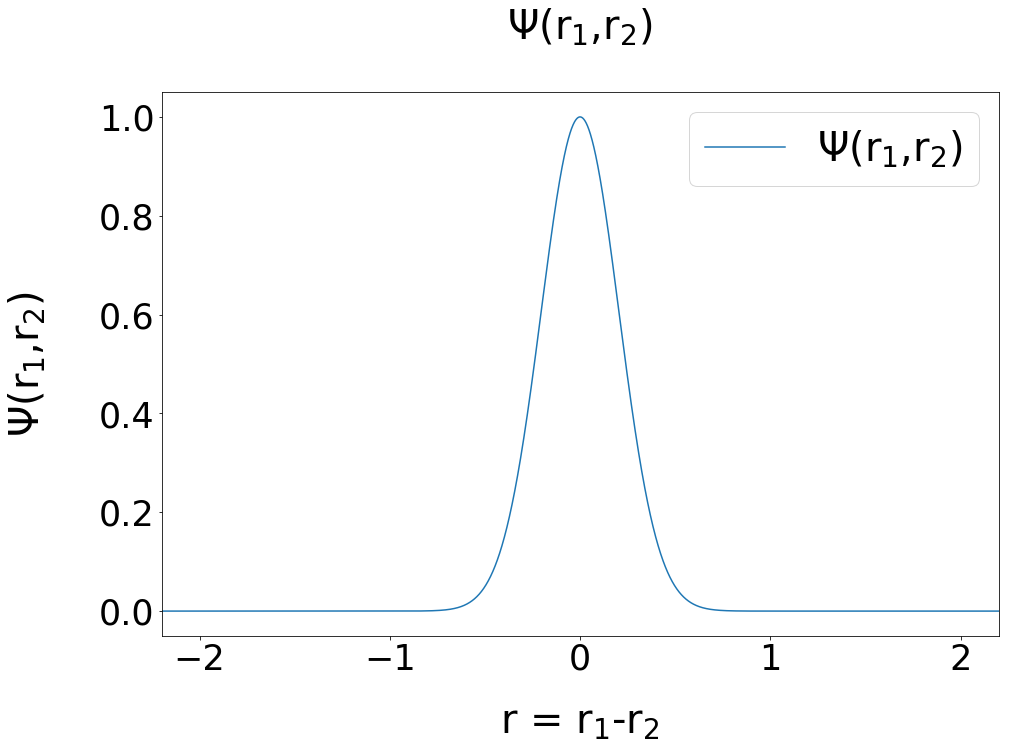
\includegraphics[scale = 0.24]{Wavefunction.png}
	\caption{\label{wavefigure} The wave function or two electrons as the product of two 1s states. The function appears to have converged to zero at r = $\pm$1 for all practical purposes.}
\end{figure}
The integrated values using the Gauss-Legendre Quadrature is plotted in figure \ref{integrated_results}.
\begin{figure}[!h]
	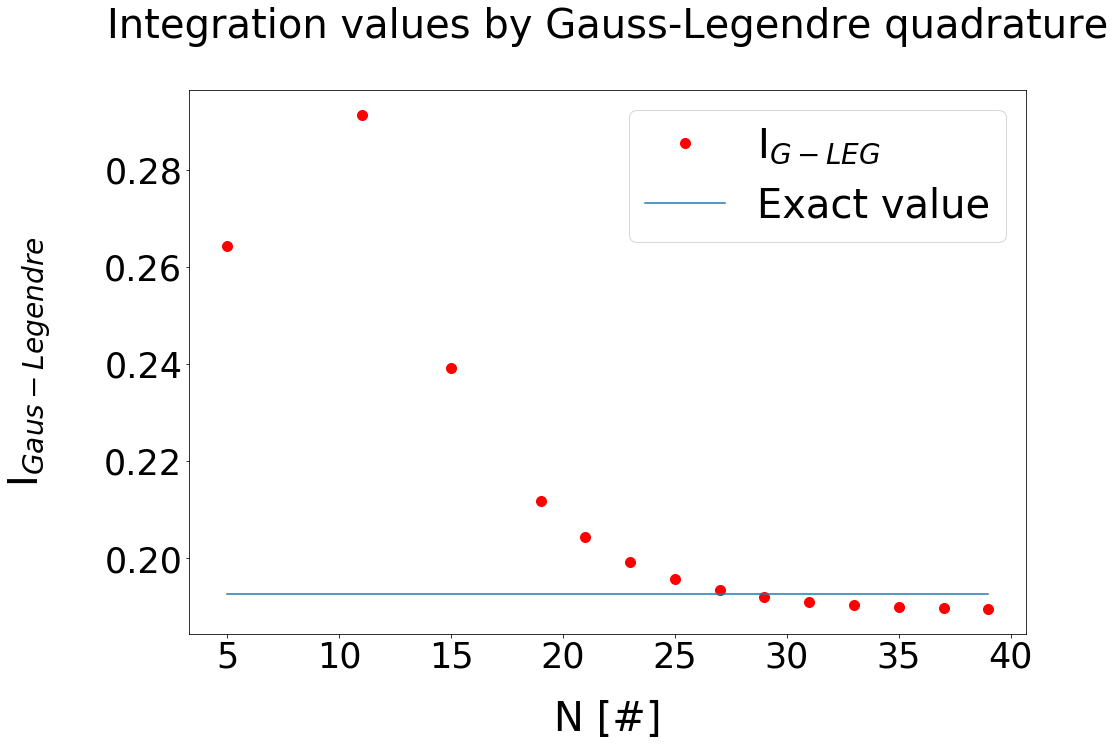
\includegraphics[scale = 0.24]{Gauss_Legendre.png}
	\caption{\label{integrated_results} The result of the Gauss-Legendre integration as a function of N}
\end{figure}

\newpage 
\section{Discussion}
\section{Conclusion }

\newpage 
\onecolumngrid
\section{Referances}
[1] Handbook of computational methods for integration, P. K. Kythe and M. R. Schaferkotter, Chapman \& Hall/CRC, Boca Raton Florida, 2005.

\section{Appendix}
\section{Tabulated values}

\begin{table}[!h]
	\begin{tabular}{|c|c|}
		\hline 
		\hspace{5mm} \textbf{N} \hspace{5mm} & \textbf{Integrated value}\\
		\hline 
		5              &        2.6425$\times 10^{-1}$             \\
		11             &        2.9126$\times 10^{-1}$               \\
		15             &        2.3909$\times 10^{-1}$               \\
		19             &        2.1183$\times 10^{-1}$               \\
		21             &        2.0431$\times 10^{-1}$               \\
		23             &        1.9923$\times 10^{-1}$               \\
		25             &        1.9582$\times 10^{-1}$               \\
		27             &        1.9352$\times 10^{-1}$               \\
		29             &        1.9199$\times 10^{-1}$               \\
		31             &        1.9099$\times 10^{-1}$               \\
		33             &        1.9033$\times 10^{-1}$               \\
		35             &        1.8992$\times 10^{-1}$               \\
		37             &        1.8968$\times 10^{-1}$               \\
		39             &        1.8956$\times 10^{-1}$               \\ \hline 
	\end{tabular}
	\caption{\label{legendre_values} The integrated value of the system using Gauss-Legendre quadrature.}
\end{table}

\newpage
\twocolumngrid

\subsubsection{Legendre Polynomials}
$P_n$ over the interval $[-1,1]$, so that $P_n(1) = 1$. If $x_{m,n}$ denotes the $m$-th zero of $P_n(x)$, where $x_{n,1} > x_{n,2} > \dots > x_{n,n} $, then 
\begin{equation}
x_{n, m}=\left(1-\frac{1}{8 n^{2}}+\frac{1}{8 n^{3}}\right) \cos \frac{(4 m-1) \pi}{4 n+2}+O\left(n^{-4}\right)
\end{equation}
The norm is equal to $2/(2n+1)$. The orthonormal legendre polynomials $p_n(x)$ are defined as 
\begin{equation}
p_{n}(x)=\sqrt{\frac{2 n+1}{2}} P_{n}(x)
\end{equation}
with the leading coefficient of $p_n(x)$ is 
\begin{equation}
a_{n}=\sqrt{\frac{2 n+1}{2}} \frac{(2 n) !}{2^{n}(n !)^{2}}
\end{equation}
It's seriesform is
\begin{equation}
P_{n}(x)=\frac{1}{2^{n}} \sum_{k=0}^{[n / 2]}(-1)^{k}\left(\begin{array}{l}{n} \\ {k}\end{array}\right)\left(\begin{array}{c}{2 n-2 k} \\ {n}\end{array}\right) x^{n-2 k}
\end{equation}
\subsubsection{Laguerre Polynomials}
For the polynomial $L_n(x)$ over the intervall $[0,\infty)$, so that $L_n(0) = n!$ and
\begin{equation}
\int_{0}^{\infty} e^{-x} L_{n}(x) L_{m}(x) d x=\left\{\begin{array}{ll}{0} & {\text { if } n \neq m} \\ {(n !)^{2}} & {\text { if } n=m}\end{array}\right.
\end{equation}
where its m-th zero $xn,m$ is given by 
\begin{equation}
x_{n, m}=\frac{j_{m}^{2}}{4 k_{n}}\left(1+\frac{j_{m}^{2}-2}{48 k_{n}^{2}}\right)+O\left(n^{-5}\right)
\end{equation}
where $k_n = n + 1/2$ and $j_m$ is the m-th positive zero of the bessel function $J_n(x)$. The norm of the polynomials is 1. 
Its series form is
\begin{equation}
L_{n}(x)=\sum_{k=0}^{n}(-1)^{k}\left(\begin{array}{c}{n} \\ {n-k}\end{array}\right) \frac{1}{k !} x^{k}
\end{equation}

\end{document}